%!TEX root = mieic.tex
\chapter{Solução Implementada} \label{chap:sol}

\section*{}

Neste capítulo é descrita de forma pormenorizada a solução implementada de modo a responder aos desafios colocados na introdução, cumprindo assim os objetivos propostos.
Inicialmente é caracterizada a arquitetura definida, fazendo referência aos diferentes modulos que constituem o “produto” final. Posteriormente são referidas de uma forma breve as tecnologias envolvidas no seu desenvolvimento.


\section{Visão Geral} \label{sec:geral}

Tal como foi referido na definição dos objetivos, era esperado o desenvolvimento e validação de uma arquitectura que permitisse uma interação baseada na manipulação direta, através de um dispositivo móvel, facilitando a criação de aplicações para ecrãs públicos.  
Na solução encontrada, de uma maneira global, é possível diferenciar três diferentes componentes, sendo eles o servidor, desenvolvido em node.js, a aplicação, que irá correr no servidor criado comunicando com este através de \textit{web sockets} e ainda o utilizador final, aqui identificado como cliente.

A figura~\ref{fig:components} apresenta, de uma forma simples, os componentes acima descritos.

\begin{figure}[ht]
\centering
\includegraphics[scale=0.62]{components.pdf}
\caption[\textit{Componentes}] {Componentes constituintes da solução desenvolvida}
\label{fig:components}
\end{figure}

A figura ~\ref{fig:sequencia} representa um diagrama de sequência mostrando as diferentes interações entre os componentes constituintes do sistema implementado. Inicialmente terá de existir um pedido por parte de um ecrã para aceder à aplicação, neste momento a aplicação comunica com o servidor e a partir daqui está preparada para pedidos de possíveis utilizadores. Um utilizador, ao querer interagir com a aplicação está a enviar um pedido para esta, que por sua vez avisa o servidor e este é responsável por mostrar no dispositivo o widget da aplicação. Neste momento o widget liga-se ao servidor e após ocorrer a ligação procede-se à troca de “mensagens” que permitem ao utilizador definir o seu nome, quando o cliente tiver o nome definido pode usufruir do widgets disponíveis, realizando-se a comunicação do  widget para o servidor, que por sua vez envia para a aplicação.

\begin{figure}[ht]
\centering
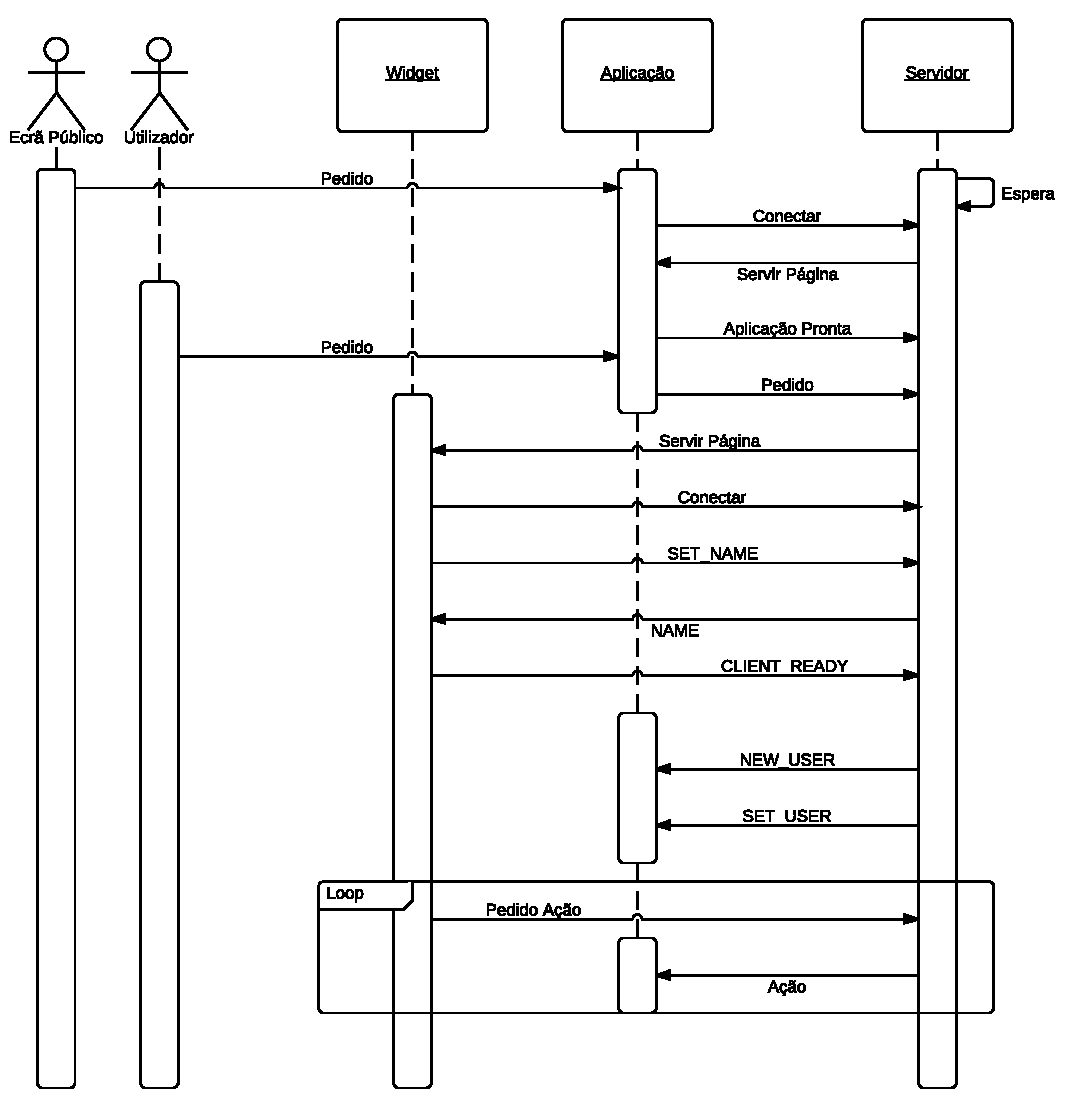
\includegraphics[scale=0.63]{Sequence.pdf}
\caption[\textit{Diagrama de Sequência}] {Diagrama de Sequência}
\label{fig:sequencia}
\end{figure}


\section{Tecnologias Usadas} \label{sec:tec}

Ao longo da implementação houve necessidade de optar por diversas tecnologias para que fosse possível alcançar o objetivo desejado, Node.js foi usado para a implementação do servidor e \textit{web sockets} e \textit{socket.io} para facilitar a comunicação entre os diversos componentes. Foi também usada a \textit{framework} \textit{Prototype} que pemrite a manipulação de classes em \textit{JavaScript}, e uma biblioteca, \textit{Swipeable} que dá resposta a eventos swipe facilitando a utilização.

\begin{itemize}

\item \textbf{Node.js}


\textit{Node.js} é uma plataforma construída para facilitar o desenvolvimento de aplicações de alta escalabilidade em tempo real, com base no interpretador \textit{Javascript V8} da \textit{Google}, que antes da execução compila \textit{JavaScript} em código máquina, melhorando consideravelmente o tempo de execução. Deste modo Node permite a construção de aplicações rápidas e altamente concorrentes.

Segundo Michael Abernethy ~\cite{Abernethy2011} node altera a noção de como um servidor deve funcionar, referindo que o seu objetivo é permitir que um programador construa applicações com grande escalabilidade e que o código desenvolvido suporte milhares de ligaçõe simultâneasa numa só máquina. 

\textit{Node.js} opera uma \textit{thread} simples, usando chamadas E/S “que não bloqueiam”(non-blocking), permitindo o suporte das diversas ligações ~\ref{fig:node}.

\begin{figure}[ht]
\centering
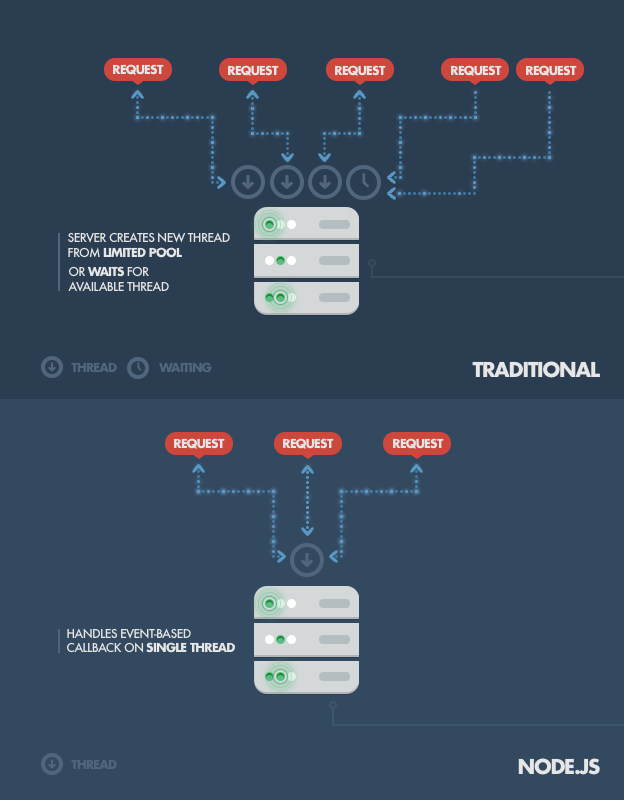
\includegraphics[width=0.5\columnwidth]{node.png}
\caption[\textit{Node.js}] {Diferença entre técnicas tradicionais de servidores e \textit{Node.js}\protect\footnotemark}
\label{fig:node}
\end{figure}

\footnotetext{http://www.toptal.com/nodejs/why-the-hell-would-i-use-node-js}

\item \textbf{Web Sockets}

De forma a permitir a comunicação do utilizador, lado do cliente, com o servidor criado foram usados web sockets. Estes foram desenvolvidos para serem implementados em em aplicações ou servidores web, usando um protocolo independente baseado em TCP.

O protocolo websocket encontra-se standardizado, o que significa que é seguida uma norma no envio de informação entre o servidor e o “browser” sem que haja uma solicitação por parte do cliente o que possibilita uma maior interação entre estes, facilitando a criação de aplicações em tempo real. É deste modo criada uma ligação bi-direcional entre o \textit{browser} e o servidor, pois a conexão é mantida aberta enquanto as mensagens são encaminhadas de um lado para o outro.


\item \textbf{Socket.io}

Socket.io é descrita como uma biblioteca javascript usada no desenvolvimento de aplicações web. Esta é composta por 2 partes, uma biblioteca para o lado do cliente, que corre no browser, e outra para o lado do servidor, que para terá de ser implementado em node.js, daí este estar acima referido como uma das tecnologias usadas. Quer o lado do cliente quer o do servidor apresentam “API’s” idênticas. 
Usa, principalmente como protocolo, websockets, também escolhido como tecnologia usada no desenvolvimento desta solução, contudo, se necessário, podem ser utilizados outros, como por exemplo Adobe Flash sockets, JSONP polling, and AJAX long polling. 
A sua escolha aliada a websockets fornece bastante recursos, como a transmissão para múltiplos sockets, armazenamento de informação associada a cada cliente e ainda “inputs/outputs” assíncronos. 

\item \textbf{Prototype}

Prototype é uma \textit{framework} em \textit{JavaScript} que fornece algumas funções para o desenvolvimento de aplicações em \textit{JavaScript}. As suas funcionalidades variam entre pequenos atalhos de programação e principais funções para lidar com \textit{XMLHttpRequest}.

Esta \textit{framework} fornece ainda uma biblioteca com funções que suporta classes e objetos baseados em classes, algo que não é possível em \textit{JavaScript}.

\item \textbf{Swipeable}

Swipeable trata-se de uma biblioteca que permite obter resposta a eventos \textit{swipe} realizados num dispositivo \textit{touch}, sendo uma abstração do \textit{touchstart}, \textit{touchmove} e \textit{touchend}. 
Foi incluída no ficheiro widget.js de para possibilitar o desenvolvimento e correto funcionamento do widget “SWIPE”.

\end{itemize}

Para além das tecnologias acima definidas todo o projeto foi realizado recorrendo a JavaScript, HTML e CSS. 


\section{Framework Desenvolvida} \label{sec:framework}

Um dos principais objetivos centrava-se no desenvolvimento de uma framework que facilitasse o desenvolvimento de aplicações para ecrãs públicos, que permitissem a manipulação direta por parte dos utilizadores, deste modo, surge a criação de uma pequena API que permite a construção e utilização de três diferentes tipos de controlo. 
Na figura~\ref{fig:classes} é representada a estrutura usada, mostrando as classes constituintes, respetivos atributos e métodos e ainda a relação entre as classes.

\begin{figure}[ht]
\centering
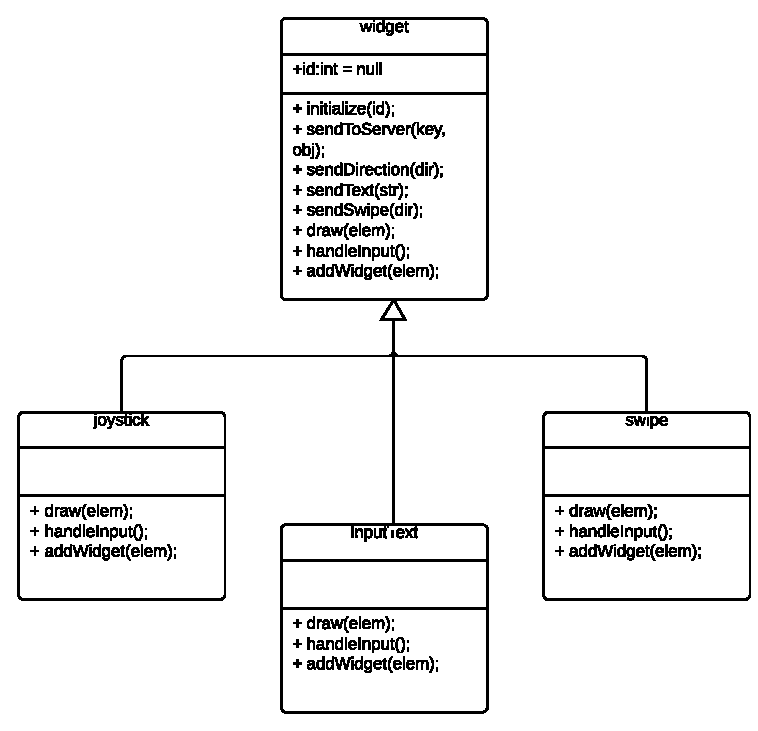
\includegraphics[scale=0.5]{classes.pdf}
\caption[\textit{classes}] {Diagrama de classes}
\label{fig:classes}
\end{figure}

A classe Widget representa uma abstração dos controlos possíveis, sendo a classe joystick, swipe e inputText instâncias desta. Uma vez que se trata de uma relação de herança, quer os atributos, quer os métodos da classe widget são herdados pelas respetivas subclasses, permitindo a sua utilização.

\subsection{Funcionalidades}

	Com o objetivo de facilitar a criação de aplicações para ecrãs públicos, foi desenvolvida uma pequena API, com um conjunto de funcionalidades que permitem a um programador o seu uso na criação de diferentes controlos de acordo ...

	A classe widget, já definida anteriormente, apresenta alguns métodos ...

	\begin{table}[ht]
 	\renewcommand{\arraystretch}{1.5}
	\centering

	\begin{tabular}{ p{2cm}|p{2cm}|p{10cm}  }
	\multicolumn{1}{c}{\textbf{Métodos}} & \multicolumn{1}{c}{\textbf{Parâmetros}} & \multicolumn{1}{c}{\textbf{Descrição}} \\
	\hline
	\multicolumn{1}{c}{initialize} & \multicolumn{1}{c}{id} &Método responsável por desenhar o widget correspondente no elemento (elem) da página html apresentada no dispositivo \\
	\hline
	\multicolumn{1}{c}{sendToServer} & \multicolumn{1}{c}{} &Método responsável por atribuir eventos aos widgets \\
	\hline
	\multicolumn{1}{c}{sendDirection} & \multicolumn{1}{c}{elem} &Método responsável por adicionar o widget à barra de widgets disponíveis no elemento, elem, da página html \\
	\hline
	\multicolumn{1}{c}{sendText} & \multicolumn{1}{c}{options} &Método que permite ao programador alterar o conteúdo do que é enviado do widget para a aplicação  \\
	\hline
	\multicolumn{1}{c}{sendSwipe} & \multicolumn{1}{c}{options} &Método que permite ao programador alterar o conteúdo do que é enviado do widget para a aplicação  \\
	\hline
	\end{tabular}
	\caption{Métodos disponíveis em cada um dos widget}
	\label{table:widget_met}
	\end{table}
	
	Os controlos referidos dizem respeito aos diferentes tipos de widget que estão disponíveis para ser usados em qualquer aplicação, e na solução apresentada disponibilizam os seguintes métodos:
	
 	\begin{table}[ht]
 	\renewcommand{\arraystretch}{1.5}
	\centering

	\begin{tabular}{ p{2cm}|p{2cm}|p{10cm}  }
	\multicolumn{1}{c}{\textbf{Métodos}} & \multicolumn{1}{c}{\textbf{Parâmetros}} & \multicolumn{1}{c}{\textbf{Descrição}} \\
	\hline
	\multicolumn{1}{c}{draw} & \multicolumn{1}{c}{elem} &Método responsável por desenhar o widget correspondente no elemento (elem) da página html apresentada no dispositivo \\
	\hline
	\multicolumn{1}{c}{handleInput} & \multicolumn{1}{c}{} &Método responsável por atribuir eventos aos widgets \\
	\hline
	\multicolumn{1}{c}{addWidget} & \multicolumn{1}{c}{elem} &Método responsável por adicionar o widget à barra de widgets disponíveis no elemento, elem, da página html \\
	\hline
	\multicolumn{1}{c}{setOptions} & \multicolumn{1}{c}{options} &Método que permite ao programador alterar o conteúdo do que é enviado do widget para a aplicação  \\
	\hline
	\end{tabular}
	\caption{Métodos disponíveis em cada um dos widget}
	\label{table:metodos}
	\end{table}


Para além dos métodos acima descritos, que constituem as opções disponíveis para a instância de cada tipo de widget, o programador tem disponíveis outros dois:

	\begin{table}[ht]
 	\renewcommand{\arraystretch}{1.5}
	\centering

	\begin{tabular}{ p{2cm}|p{2cm}|p{10cm}  }
	\multicolumn{1}{c}{\textbf{Método}} & \multicolumn{1}{c}{\textbf{Parâmetros}} & \multicolumn{1}{c}{\textbf{Descrição}} \\
	\hline
	\multicolumn{1}{c}{start} & \multicolumn{1}{c}{url, options} &Método para inicializar o widgets, responsável por efetuar a ligação com o servidor \\
	\hline
	\multicolumn{1}{c}{drawBar} & \multicolumn{1}{c}{elem} &Método por desenhar, no elemento, elem, da página html, a barra que mostra ao utilizador os widgets que tem disponíveis \\
	\hline
	\end{tabular}
	\caption{Métodos}
	\label{table:metodos_g}
	\end{table}



\subsection{Controlos Definidos}

	A API desenvolvida apresenta três diferentes tipos de controlos que o programador terá à sua disposição para implementar, de acordo com aplicação desenvolvida. Neste momento existem como possíveis opções, o \textit{joystick}, o \textit{swipe} e ainda outro composto por uma caixa de introdução de texto.

	\begin{itemize}

	\item \textbf{Joystick}

		Controlo composto pelas quatro setas tradicionais, esquerda, direita, cima e baixo, que pode ser utilizado em qualquer aplicação que exija uma movimentação.

		\begin{figure}[ht]
		\centering
		
\includegraphics[scale=0.6]{joystick.png}
		\caption[\textit{Widget Joystick}] {\textit{Widget Joystick}}
		\label{fig:joystick}
		\end{figure}
		

	\item \textbf{Swipe}

		Controlo que usa as propriedade touch do dispositivo para controlar a aplicação, definido apenas para reconhecer uma direção, contudo pode ser alterado.

		\begin{figure}[ht]
		\centering
		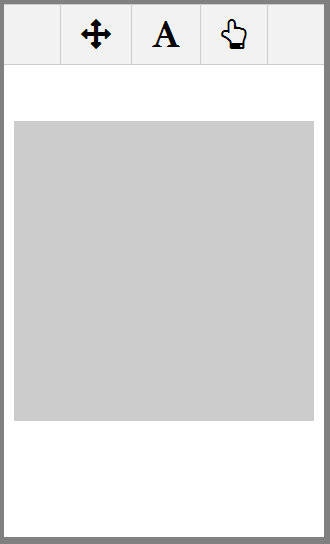
\includegraphics[scale=0.6]{swipe.png}
		\caption[\textit{Widget Swipe}] {\textit{Widget Swipe}}
		\label{fig:swipe}
		\end{figure}

	\item \textbf{InputText}

		Controlo que permite ao utilizador a interação com aplicações que exijam a introdução de texto.

		\begin{figure}[ht]
		\centering
		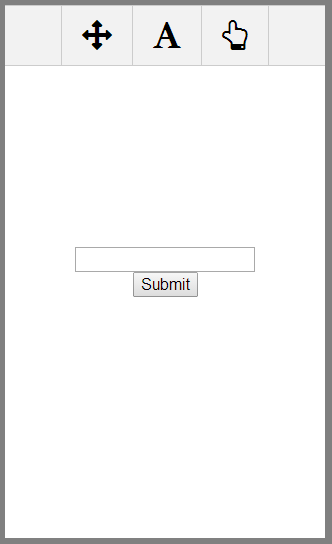
\includegraphics[scale=0.6]{text.png}
		\caption[\textit{Widget Input Text}] {\textit{Widget Input Text}}
		\label{fig:text}
		\end{figure}

	\end{itemize}

\subsection{Utilização}

	O principal pressuposto do desenvolvimento desta API é permitir que um programador, possa, mais facilmente, desenvolver aplicações para ecrãs públicos, preocupando-se apenas com os controlos que estas necessitam.
	Para a correta utilização, de acordo com o trabalho realizado, o programador terá de criar um ficheiro .html, cujo nome seja widget.html, onde deverá incluir a biblioteca widget.js, sendo esta dependente de outras bibliotecas que terão de ser incluídas no mesmo ficheiro, como \textit{Socket.io}, \textit{prototype} e \textit{swipeable}. 

	
\section{Aplicação Implementada} \label{sec:exemplo}

	Neste momento apenas existe uma aplicação exemplo, no entanto permite ao utilizador o uso dos três tipos de controlo disponíveis. 

	No trabalho apresentado, o clássico jogo \textit{Snake}, surge como o exemplo citado, no qual o utilizador é obrigado a inserir o seu nome, usando para isso a opção de introdução de texto e só posteriormente poderá escolher entre o \textit{joystick} ou o \textit{swipe}, servindo qualquer um deles para controlar a direção da cobra durante o jogo. Cabe ao utilizador a escolha do controlo adequado de acordo com as suas preferências ou facilidades, necessitando apenas de carregar na barra superior no botão correspondente ao \textit{widget} desejado.

	\subsection{Ligação}

	Tendo em conta que a aplicação funcionará num ecrã público, e que é suposto o transeunte usufruir da mesma através do seu dispositivo móvel, é necessário que exista um método que permita a ligação entre os dois.

	Na solução implementada, esta ligação ocorre através da leitura de um \textit{qr code}, que se encontra sempre disponível no ecrã.

	\subsection{Feedback da aplicação}

	Uma vez que se trata de uma interação pública com a qual uma ou mais pessoas devem poder interagir, é importante que durante a sua utilização, a pessoa que se esta a servir desta, seja capaz de perceber o fluxo de informação que ocorre entre ela e a aplicação. Como por exemplo, conseguir identificar-se quando existem mais do que um utilizador e ainda perceber em que momento pode começar a interagir.

	No exemplo implementado, sempre que uma nova pessoa se conecta com o jogo o servidor lança um alerta, aparecendo uma notificação de como existe um novo jogador em condições usufruir da aplicação presente. 
	\missingfigure{notificação de entrada}

	Quem desejar interagir com a solução implementada necessita de introduzir um nome de utilizador, antes de realmente poder jogar, no ecrã surgirá então o nome escolhido, que, neste caso concreto, uma vez que é um jogo, o nome surge acompanhado dos pontos conseguidos, e vai sendo atualizado à medida que são alterados.
	\missingfigure{nome utilizador}

	\subsection{Distinção de utilizadores}

	Numa aplicação que permita o seu uso por mais do que uma pessoa é importante ter em conta de que modo é feita a distinção entre os diversos utilizadores, percebendo que cada um dos intervenientes terá de se reconhecer durante o momento da interação. 

	No jogo implementado, tal como foi referido no ponto anterior o jogador é identificado pelo nome que este escolhe quando se conecta com o ecrã, no entanto há ainda a necessidade deste se reconhecer na aplicação que está no momento a utilizar. A solução encontrada, no contexto do exemplo usado, passou por colorir o nome do jogador com a cor da cobra que o representa durante o jogo, permitindo assim a distinção dos jogadores e transmitindo-lhes quem é quem no jogo que está a decorrer.
	\missingfigure{nomes coloridos}

	\subsection{Como utilizar}

	Enquanto utilizador final, para poder utilizar a aplicação desenvolvida será necessário:
	\begin{itemize}
		\item Possuir um dispositivo com acesso a internet;
		\item Ter um \textit{browser} instalado;
		\item Ter instalada no seu dispositivo uma aplicação que permita a leitura de \textit{QR codes}.
	\end{itemize}

	O diagrama seguinte, ilustra, de forma sequencial os passos existentes numa interação com a aplicação.
	\newline

	\begin{figure}[ht]
	\centering
	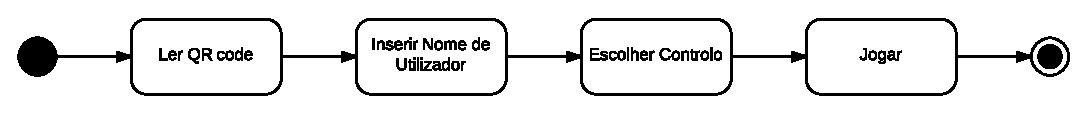
\includegraphics[width=\linewidth]{activity.pdf}
	\caption[Utilização]{Interação com a aplicação}
	\label{fig:interagir}
	\end{figure}

	Ao aproximar-se de um ecrã que tenha a correr este exemplo, o transeunte deve:

	\begin{enumerate}
		\item Ler o \textit{QR code} presente no ecrã;
		\item Introduzir um nome pelo qual quer ser identificado;
		\item Escolher o controlo desejado para jogar;
		\item Jogar.
	\end{enumerate}


	


	





